\section{Aufgabe 3} \label{ex3}
Der Farbbereich wurde nun auf 16Bit pro Farbe erweitert.\\
Zusätzlich können über die Hardware-Switches drei verschiedene Modi umgeschaltet werden:\\

BTN0: Toggle Augenfarbe zwischen rot und blau\\
BTN1: Toggle Random Walker\\
BTN2: Hintergrundfarbe umschalten zwsichen blau/\textbf{grau}

\subsection{VHDL 12Bit Update VGA-Controller}
VHDL Code mit Erweiterung des RAM Speichers auf 12 Bit um RGB je mit 4 Bits (16 Farben) verarbeiten zu können:
\begin{verbatim}
-------------------------------------------------------------
-- RAM auf 12 Bit pro Speicheradresse erweitert
-------------------------------------------------------------
  constant low_address: natural := 0;
    constant high_address: natural := ((640 * 480) - 1);
     -- 640 * 480 =  307200 --> Starten bei 0 --> 307199
    -- TYPE ram_type is array (high_address downto low_address) of 
    -- std_logic_vector (11 downto 0);
    SIGNAL RAM: ram_type;

 -- The current Ram Adress
    signal RAM_address : integer RANGE low_address TO high_address := low_address;
    -- The current Ram Data  
    signal ram_Data    : std_logic_vector(11 downto 0) := "000000000000"; 
-------------------------------------------------------------
-- process um den RAM zu lesen wurde erweitert
-------------------------------------------------------------
  process(vga_clk)      
        begin
        if falling_edge(vga_clk) then
            if (video_on='1') then
                -- vga_colour_out <= ram_Data;     
                  
                red    <=  ram_Data(11 downto 8);
                green   <= ram_Data(7 downto 4);
                blue    <= ram_Data(3 downto 0);
            else
                red   <= (others => '0');
                green <= (others => '0');
                blue  <= (others => '0');
            end if;
            hSync <= hsynct;
            vSync <= vsynct;
        end if;
    end process; 
\end{verbatim}

\subsection{C-Code 12Bit Update VGA-Controller}
Auch wurde der C-Code auf 12 Bit Farben erweitert: 
\begin{verbatim}
/* This application configures UART 16550 to baud rate 9600.
 * PS7 UART (Zynq) is not initialized by this application, since
 * bootrom/bsp configures it to baud rate 115200
 *
 * ------------------------------------------------
 * | UART TYPE   BAUD RATE                     |
 * ------------------------------------------------
 *   uartns550   9600
 *   uartlite    Configurable only in HW design
 *   ps7_uart    115200 (configured by bootrom/bsp)
 */
#include  <stdio.h>
#include  <stdlib.h>
#include  <time.h>

#include "platform.h"
//  Include  Files
#include "xparameters.h"
#include "xgpio.h"
#include "xstatus.h"
#include "xil_printf.h"
#include "lab3_a1_vga_v2.h"

//  Definitions
#define BASE_ADDR 0x43C00000
//#define  LEDS_DEVICE_ID  XPAR_AXI_GPIO_0_DEVICE_ID
#define  SW_DEVICE_ID  XPAR_AXI_GPIO_0_DEVICE_ID

#define  LED_DELAY  10000000
#define  LED_CHANNEL 1
#define  printf  xil_printf

XGpio  SWInst; // LEDInst
static int sw_value ;

#define BTN0 1
#define BTN1 2
#define BTN2 4
#define BTN3 8
#define BTN4 16
#define BTN5 32
#define BTN6 64
#define BTN7 128

#define EYE 2
#define BODY 46

// predifined colors
typedef enum _color {
		eS = 0b000000000000,
		eW = 0b111111111111,
	eWgray = 0b011001100110,
		eR = 0b111100000000,
	eRdark = 0b011100000000,
		eG = 0b000011110000,
	eGdark = 0b000001110000,
		eB = 0b000000001111,
	eBdark = 0b000000000111
} ecolor;

typedef struct _coord {
	int x;
	int y;
} coord;

// Arcade figure
uint eyex[EYE] = {3,7};
uint eyey[EYE] = {3,3};
uint spx[BODY] = {2,8,3,7, 2,3,4,5,6,7,8, 1,2,4,5,6,8,9, 
                   0,1,2,3,4,5,6,7,8,9,10, 0,2,3,4,5,6,7,8,10, 0,2,8,10, 3,4,6,7};
uint spy[BODY] = {0,0,1,1, 2,2,2,2,2,2,2, 3,3,3,3,3,3,3, 
                   4,4,4,4,4,4,4,4,4,4, 4, 5,5,5,5,5,5,5,5, 5, 6,6,6, 6, 7,7,7,7};

void paintsquare(uint x, uint y, uint size, ecolor color) {
	if (x < 0 || x > 630)
		return;
	if (y < 0 || y > 470)
		return;
		
	uint i,j;
	for (i = x; i < x+size; ++i)
		for (j = y; j < y+size; ++j)
			LAB3_A1_VGA_V2_mWriteReg((u32)BASE_ADDR, 0, (i << 21 | j << 12 | color));
} 

void resetbg (ecolor color) {
	int i,j;
	for (i = 0; i < 680; ++i)
		for (j = 0; j < 480; ++j)
			LAB3_A1_VGA_V2_mWriteReg((u32)BASE_ADDR, 0, (i << 21 | j << 12 | color));
}

int  main()
{
	double DELAY = 10000000,z;
	srand(5637);
	init_platform ();
	int status ;

	// Initialise Push Buttons
	status = XGpio_Initialize (&SWInst , SW_DEVICE_ID );
	if ( status != XST_SUCCESS )
		return XST_FAILURE ;

	// Set LEDs direction to outputs
	//XGpio_SetDataDirection (&LEDInst,1,0x00);
	// Set all switches direction to inputs
	XGpio_SetDataDirection (&SWInst,1,0xFF);

	print("Hello world\n\r");

	//SWReadExample ();
	uint i,j;
	coord pos = {100,100};
	coord pos_new = {100,100};
	
	uint write_new = 1;
	uint delete = 0;
	uint background_repaint = 0;

	uint size = 10;
	ecolor color = eR;
	uint btn0_on = 0, btn1_on = 0, btn2_on = 0;

	ecolor bgcolor = eWgray;
	resetbg(bgcolor);

	while (1) {

		sw_value = XGpio_DiscreteRead (&SWInst , 1);

		/* toggle eye color */
		if (btn0_on != (sw_value & BTN0) ) {
			write_new = 1;
			btn0_on = sw_value & BTN0;

			if (btn0_on == BTN0)
				color = eB;
			else
				color = eR;
		}
		
		// random walker
		if ( sw_value & BTN1 && write_new == 0 ) {
			//xil_printf ("Switch 1 active!!!: %x\n\r",sw_value);

			for (z = 0; z<DELAY;z+=1)
				delete = 1;

			write_new = 60;
			uint dir = rand() % 7;
			switch (dir) {
			case 0:
				// up
				pos_new.x = 0;
				pos_new.y =-2;
				break;
			case 1:
				// up right
				pos_new.x = 1;
				pos_new.y = -1;
				break;
			case 2:
				// right
				pos_new.x = 2;
				pos_new.y = 0;
				break;
			case 3:
				// right down
				pos_new.x = 1;
				pos_new.y = 1;
				break;
			case 4:
				// down
				pos_new.x = 0;
				pos_new.y = 2;
				break;
			case 5:
				// down left
				pos_new.x = -1;
				pos_new.y = 1;
				break;
			case 6:
				// left
				pos_new.x = -2;
				pos_new.y = 0;
				break;
			case 7:
				// up left
				pos_new.x = -1;
				pos_new.y = -1;
				break;
			default:
				break;
			}
		}

		/* toggle bg color */
		if (btn2_on != (sw_value & BTN2) ) {
			write_new = 1;
			btn2_on = sw_value & BTN2;

			xil_printf ("Switch 2: %x\n\r",(sw_value & BTN2));
			if (btn2_on == BTN2) {
				xil_printf ("Switch 2 = 1: %d\n\r",1);
				bgcolor = eBdark;
				resetbg(bgcolor);
			}
			else {
				bgcolor = eWgray;
				resetbg(bgcolor);
			}
		}

		if (delete) {
			// do we need wait statements to not write too fast to the FPGA
			for (i = 0; i < EYE; ++i)
				paintsquare(pos.x + size*eyex[i], pos.y + size*eyey[i], size, bgcolor);
			for (i = 0; i < BODY; ++i)
				paintsquare(pos.x + size*spx[i], pos.y + size*spy[i], size, bgcolor);

			if ((pos.x + pos_new.x) > 0 && (pos.x + pos_new.x) < 530 )
				pos.x += pos_new.x;
			if ((pos.y + pos_new.y) > 0 && (pos.y + pos_new.y) < 400 )
				pos.y += pos_new.y;

			delete = 0;
		}

		if (write_new) {
			// do we need wait statements to not write too fast to the FPGA
			for (i = 0; i < EYE; ++i)
				paintsquare(pos.x + size*eyex[i], pos.y + size*eyey[i], size, color);
			for (i = 0; i < BODY; ++i)
				paintsquare(pos.x + size*spx[i], pos.y + size*spy[i], size, eG);
			
			write_new--;
		}
		
		//sleep(1);

	}; // while

	cleanup_platform ();
	return  0;
}
\end{verbatim}

Nun kann der Hintergrund auf grau geändert werden. Hierzu werden alle drei Farben 
gemischt (eWgray = 0b0110 0110 0110) also je 6 Bit von 16 gesetzt 0x666 (RGB).\\

\begin{minipage}{\textwidth}
    \begin{center}        
        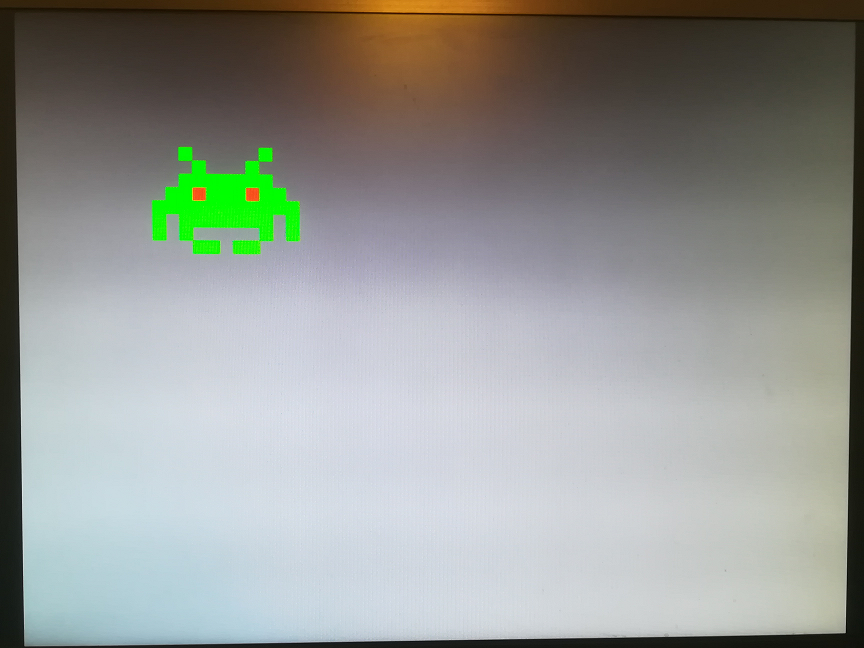
\includegraphics[scale=0.5]{img/green.png} 
    \end{center}
\end{minipage}
\begin{center}
Arcade-SpaceInvader mit grauem Hintergrund
\end{center}

\section{Debugging via Serial Interface}

Im Vivado Interface kann die Serielle Schnittstelle komfortable angezeigt werden. Dazu wird ein USB-Kabel  an den 
Port \textbf{s} (siehe Kap.2.) und im Geräte Manager der entsprechende Port herausgesucht.\\

\begin{minipage}{\textwidth}
    \begin{center}        
        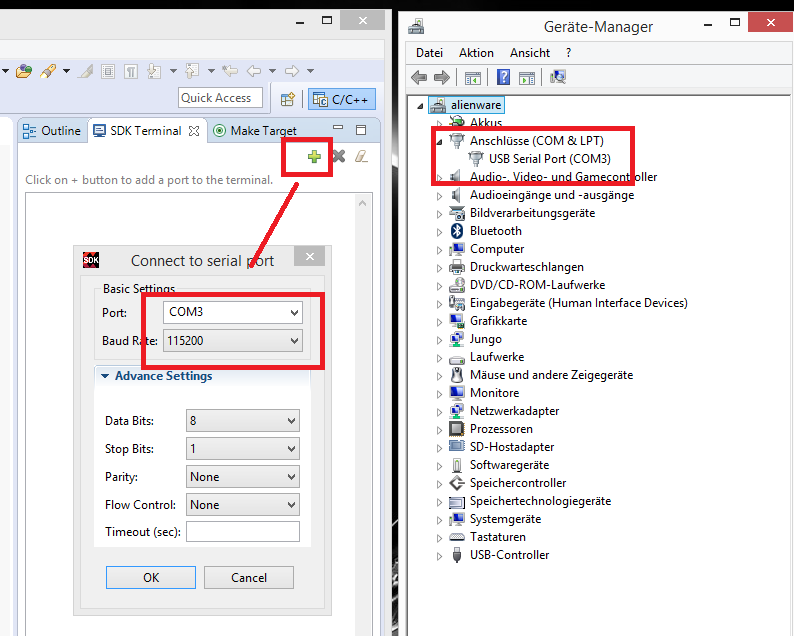
\includegraphics[scale=0.5]{img/vivadosdk_serial.png} 
    \end{center}
\end{minipage}
\begin{center}
Vivado SDK-Termial
\end{center}





